\documentclass[14pt]{extbook}
\usepackage{multicol, enumerate, enumitem, hyperref, color, soul, setspace, parskip, fancyhdr} %General Packages
\usepackage{amssymb, amsthm, amsmath, latexsym, units, mathtools} %Math Packages
\everymath{\displaystyle} %All math in Display Style
% Packages with additional options
\usepackage[headsep=0.5cm,headheight=12pt, left=1 in,right= 1 in,top= 1 in,bottom= 1 in]{geometry}
\usepackage[usenames,dvipsnames]{xcolor}
\usepackage{dashrule}  % Package to use the command below to create lines between items
\newcommand{\litem}[1]{\item#1\hspace*{-1cm}\rule{\textwidth}{0.4pt}}
\pagestyle{fancy}
\lhead{Progress Quiz 9}
\chead{}
\rhead{Version C}
\lfoot{9541-5764}
\cfoot{}
\rfoot{Summer C 2021}
\begin{document}

\begin{enumerate}
\litem{
Construct the lowest-degree polynomial given the zeros below. Then, choose the intervals that contain the coefficients of the polynomial in the form $ax^3+bx^2+cx+d$.\[ \frac{4}{3}, \frac{2}{3}, \text{ and } \frac{3}{5} \]\begin{enumerate}[label=\Alph*.]
\item \( a \in [43, 49], b \in [-121, -109], c \in [94, 102], \text{ and } d \in [-30, -23] \)
\item \( a \in [43, 49], b \in [115, 126], c \in [94, 102], \text{ and } d \in [24, 25] \)
\item \( a \in [43, 49], b \in [2, 5], c \in [-61, -52], \text{ and } d \in [24, 25] \)
\item \( a \in [43, 49], b \in [63, 65], c \in [-21, -6], \text{ and } d \in [-30, -23] \)
\item \( a \in [43, 49], b \in [-121, -109], c \in [94, 102], \text{ and } d \in [24, 25] \)

\end{enumerate} }
\litem{
Describe the end behavior of the polynomial below.\[ f(x) = 8(x - 9)^{5}(x + 9)^{10}(x - 3)^{3}(x + 3)^{5} \]\begin{enumerate}[label=\Alph*.]
\begin{multicols}{2}\item 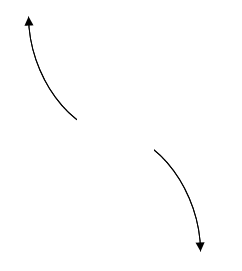
\includegraphics[width = 0.3\textwidth]{../Figures/polyEndBehaviorCopyAC.png}\item 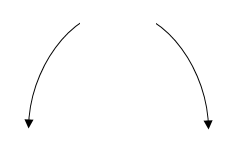
\includegraphics[width = 0.3\textwidth]{../Figures/polyEndBehaviorCopyBC.png}\item 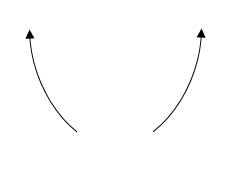
\includegraphics[width = 0.3\textwidth]{../Figures/polyEndBehaviorCopyCC.png}\item 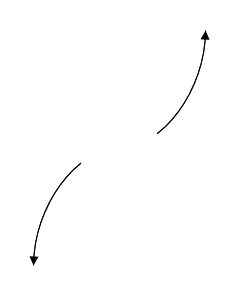
\includegraphics[width = 0.3\textwidth]{../Figures/polyEndBehaviorCopyDC.png}\end{multicols}\item None of the above.
\end{enumerate} }
\litem{
Construct the lowest-degree polynomial given the zeros below. Then, choose the intervals that contain the coefficients of the polynomial in the form $x^3+bx^2+cx+d$.\[ 2 + 4 i \text{ and } 1 \]\begin{enumerate}[label=\Alph*.]
\item \( b \in [4.8, 7.3], c \in [22.72, 24.73], \text{ and } d \in [18.8, 23.2] \)
\item \( b \in [-0.5, 1.6], c \in [-4.03, -2.68], \text{ and } d \in [0.5, 2.3] \)
\item \( b \in [-8.6, -2.1], c \in [22.72, 24.73], \text{ and } d \in [-21.3, -19.8] \)
\item \( b \in [-0.5, 1.6], c \in [-5.22, -3.99], \text{ and } d \in [2.7, 7] \)
\item \( \text{None of the above.} \)

\end{enumerate} }
\litem{
Which of the following equations \textit{could} be of the graph presented below?
\begin{center}
    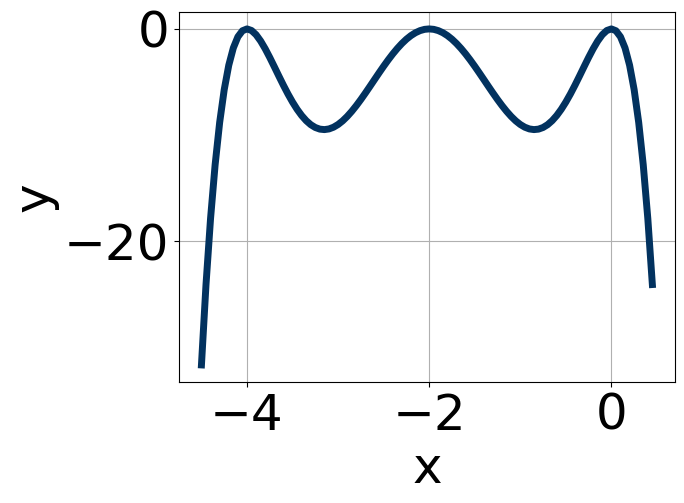
\includegraphics[width=0.5\textwidth]{../Figures/polyGraphToFunctionCopyC.png}
\end{center}
\begin{enumerate}[label=\Alph*.]
\item \( 18x^{5} (x + 2)^{8} (x + 4)^{4} \)
\item \( 9x^{10} (x + 2)^{8} (x + 4)^{6} \)
\item \( -6x^{5} (x + 2)^{8} (x + 4)^{6} \)
\item \( -3x^{4} (x + 2)^{8} (x + 4)^{8} \)
\item \( -14x^{5} (x + 2)^{6} (x + 4)^{5} \)

\end{enumerate} }
\litem{
Describe the zero behavior of the zero $x = 9$ of the polynomial below.\[ f(x) = 9(x - 3)^{11}(x + 3)^{8}(x - 9)^{10}(x + 9)^{9} \]\begin{enumerate}[label=\Alph*.]
\begin{multicols}{2}\item 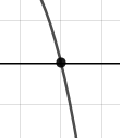
\includegraphics[width = 0.3\textwidth]{../Figures/polyZeroBehaviorCopyAC.png}\item 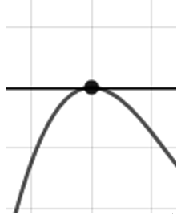
\includegraphics[width = 0.3\textwidth]{../Figures/polyZeroBehaviorCopyBC.png}\item 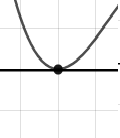
\includegraphics[width = 0.3\textwidth]{../Figures/polyZeroBehaviorCopyCC.png}\item 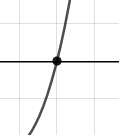
\includegraphics[width = 0.3\textwidth]{../Figures/polyZeroBehaviorCopyDC.png}\end{multicols}\item None of the above.
\end{enumerate} }
\litem{
Describe the zero behavior of the zero $x = 4$ of the polynomial below.\[ f(x) = 5(x + 6)^{5}(x - 6)^{4}(x + 4)^{9}(x - 4)^{6} \]\begin{enumerate}[label=\Alph*.]
\begin{multicols}{2}\item 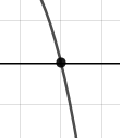
\includegraphics[width = 0.3\textwidth]{../Figures/polyZeroBehaviorAC.png}\item 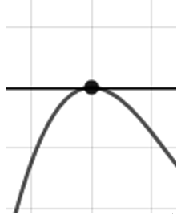
\includegraphics[width = 0.3\textwidth]{../Figures/polyZeroBehaviorBC.png}\item 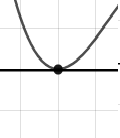
\includegraphics[width = 0.3\textwidth]{../Figures/polyZeroBehaviorCC.png}\item 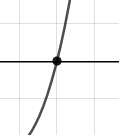
\includegraphics[width = 0.3\textwidth]{../Figures/polyZeroBehaviorDC.png}\end{multicols}\item None of the above.
\end{enumerate} }
\litem{
Describe the end behavior of the polynomial below.\[ f(x) = 2(x + 4)^{3}(x - 4)^{8}(x - 5)^{5}(x + 5)^{6} \]\begin{enumerate}[label=\Alph*.]
\begin{multicols}{2}\item 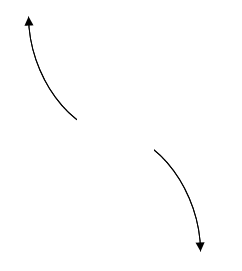
\includegraphics[width = 0.3\textwidth]{../Figures/polyEndBehaviorAC.png}\item 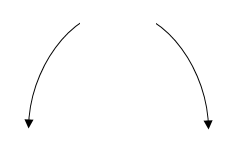
\includegraphics[width = 0.3\textwidth]{../Figures/polyEndBehaviorBC.png}\item 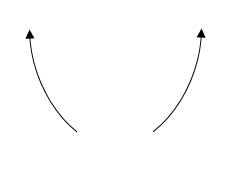
\includegraphics[width = 0.3\textwidth]{../Figures/polyEndBehaviorCC.png}\item 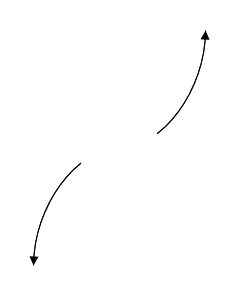
\includegraphics[width = 0.3\textwidth]{../Figures/polyEndBehaviorDC.png}\end{multicols}\item None of the above.
\end{enumerate} }
\litem{
Construct the lowest-degree polynomial given the zeros below. Then, choose the intervals that contain the coefficients of the polynomial in the form $x^3+bx^2+cx+d$.\[ -4 - 3 i \text{ and } 1 \]\begin{enumerate}[label=\Alph*.]
\item \( b \in [-2.3, 1.9], c \in [1.81, 2.56], \text{ and } d \in [-3.42, -2.96] \)
\item \( b \in [-8.3, -5.2], c \in [15.94, 17.54], \text{ and } d \in [24.44, 26.01] \)
\item \( b \in [4.9, 8.8], c \in [15.94, 17.54], \text{ and } d \in [-26.86, -23.36] \)
\item \( b \in [-2.3, 1.9], c \in [2.49, 3.29], \text{ and } d \in [-4.03, -3.82] \)
\item \( \text{None of the above.} \)

\end{enumerate} }
\litem{
Construct the lowest-degree polynomial given the zeros below. Then, choose the intervals that contain the coefficients of the polynomial in the form $ax^3+bx^2+cx+d$.\[ \frac{-7}{4}, \frac{7}{2}, \text{ and } \frac{-3}{5} \]\begin{enumerate}[label=\Alph*.]
\item \( a \in [33, 45], b \in [-46, -44], c \in [-295, -277], \text{ and } d \in [-147, -143] \)
\item \( a \in [33, 45], b \in [90, 98], c \in [-205, -195], \text{ and } d \in [-147, -143] \)
\item \( a \in [33, 45], b \in [35, 50], c \in [-295, -277], \text{ and } d \in [146, 151] \)
\item \( a \in [33, 45], b \in [-186, -184], c \in [111, 127], \text{ and } d \in [146, 151] \)
\item \( a \in [33, 45], b \in [-46, -44], c \in [-295, -277], \text{ and } d \in [146, 151] \)

\end{enumerate} }
\litem{
Which of the following equations \textit{could} be of the graph presented below?
\begin{center}
    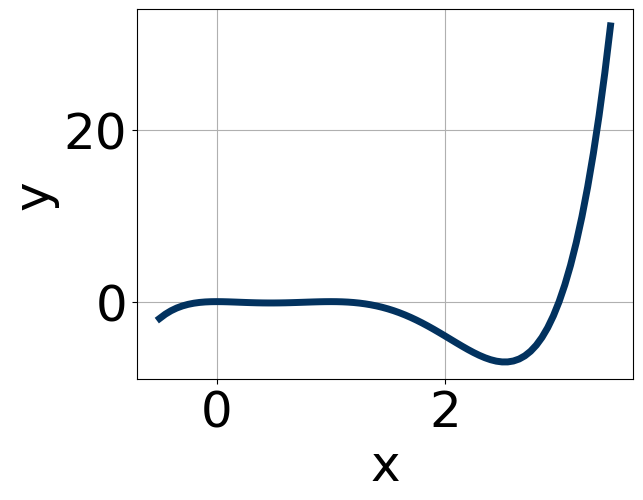
\includegraphics[width=0.5\textwidth]{../Figures/polyGraphToFunctionC.png}
\end{center}
\begin{enumerate}[label=\Alph*.]
\item \( 6x^{9} (x - 1)^{4} (x - 3)^{5} \)
\item \( 19x^{11} (x - 1)^{8} (x - 3)^{6} \)
\item \( 9x^{4} (x - 1)^{10} (x - 3)^{9} \)
\item \( -8x^{10} (x - 1)^{8} (x - 3)^{7} \)
\item \( -11x^{4} (x - 1)^{8} (x - 3)^{8} \)

\end{enumerate} }
\end{enumerate}

\end{document}